\documentclass{article}

% Language setting
% Replace `english' with e.g. `spanish' to change the document language
\usepackage[english]{babel}

% Set page size and margins
% Replace `letterpaper' with `a4paper' for UK/EU standard size
\usepackage[letterpaper,top=0.5cm,bottom=0.5cm,left=0.5cm,right=0.5cm,marginparwidth=1
0cm]{geometry}

% Useful packages
\usepackage{amsmath}
\usepackage{graphicx}
\usepackage[table]{xcolor}
\usepackage[colorlinks=true, allcolors=blue]{hyperref}
\usepackage{pdflscape}
\usepackage{tikz}
\usetikzlibrary{arrows,arrows.meta,shapes,positioning,shadows,trees}

\usepackage[
backend=biber,
style=ieee,
]{biblatex}


\addbibresource{sample.bib} %Imports bibliography file

\begin{document}


% ---------------------------
% Title page (custom)
% ---------------------------
\begin{titlepage}
  \begin{center}
    \includegraphics[width=5cm]{nup_logo.png} \\[1cm]
    {\Large Neapolis University Pafos} \\[0.5cm]

    {\large \textbf{Course Code:} IS506} \\[2cm]

    {\huge \textbf{IT Project Management Midterm}} \\[1.5cm]

    {\large \textbf{Name:} Aleksandr Petrunin} \\[0.3cm]
    {\large \textbf{Student ID:} 1251114137} \\[2cm]

    {\large \today}
  \end{center}
\end{titlepage}

\begin{landscape}
\section{Q1 (40 points)}

\tikzset{
  basic/.style  = {draw, text width=2cm, drop shadow, font=\sffamily, rectangle},
  root/.style   = {basic, rounded corners=2pt, thin, align=center,
                   fill=green!30},
  level 2/.style = {basic, rounded corners=6pt, thin,align=center, fill=green!60,
                   text width=8em},
  level 3/.style = {basic, thin, align=left, fill=yellow!60, text width=7em},
  level4/.style = {basic, thin, align=left, fill=pink!60, text width=7em}
}

\begin{tikzpicture}[
  level 1/.style={sibling distance=45mm},
  edge from parent/.style={->,draw},
  >=latex]

% root of the the initial tree, level 1
\node[root] {Mobile Banking App WBS}
% The first level, as children of the initial tree
  child {node[level 2] (c1) {1. Requirements}}
  child {node[level 2] (c2) {2. Design}}
  child {node[level 2] (c3) {3. Development}}
  child {node[level 2] (c4) {4. Testing}}
  child {node[level 2] (c5) {5. Deployment}}
  child {node[level 2] (c6) {6. Pr.Management}};

  % The second level, relatively positioned nodes
\begin{scope}[every node/.style={level 3}]
\node [below of = c1, xshift=15pt] (c11) {1.1 Stakeholder interviews};
\node [below of = c11, yshift=-120pt] (c12) {1.2 Feature set listing};
\node [below of = c12, yshift=-120pt] (c13) {1.3 Feature set prioritization};

\node [below of = c2, xshift=15pt] (c21) {2.1 UX};
\node [below of = c21, yshift=-120pt] (c22) {2.2 Design System};
\node [below of = c22, yshift=-120pt] (c23) {2.3 UI};

\node [below of = c3, xshift=15pt] (c31) {3.1 API implementation};
\node [below of = c31, yshift=-120pt] (c32) {3.2 App Backend};
\node [below of = c32, yshift=-120pt] (c33) {3.3 App Frontend};

\node [below of = c4, xshift=15pt] (c41) {4.1 Unit testing};
\node [below of = c41, yshift=-120pt] (c42) {4.2 Integration testing};
\node [below of = c42, yshift=-120pt] (c43) {4.3 Regression testing};
\node [below of = c5, xshift=15pt] (c51) {5.1 GitOps infrastructure};
\node [below of = c51, yshift=-120pt] (c52) {5.2 Development stage};
\node [below of = c52, yshift=-75pt] (c53) {5.3 Staging environment};
\node [below of = c53, yshift=-100pt] (c54) {5.4 Production stage};

\node [below of = c6, xshift=15pt] (c61) {6.1 Resources};
\node [below of = c61, yshift=-120pt] (c62) {6.2 Timeline};
\node [below of = c62, yshift=-120pt] (c63) {6.3 Risks};
\end{scope}

% The third level
\begin{scope}[every node/.style={level4}]
\node [below of = c11, xshift=15pt] (c111) {1.1.1 Conduct 3+ interviews};
\node [below of = c111, yshift=-5pt] (c112) {1.1.2 Cover gaps and needs};
\node [below of = c112, yshift=-5pt] (c113) {1.1.3 Create knowledge base};

\node [below of = c12, xshift=15pt] (c121) {1.2.1 Non-functional};
\node [below of = c121, yshift=-5pt] (c122) {1.2.2 Functional};

\node [below of = c13, xshift=15pt] (c131) {1.3.1 MOST analysis};
\node [below of = c131, yshift=-5pt] (c132) {1.3.2 SWOT analysis};
\node [below of = c132, yshift=-5pt] (c133) {1.3.3 MoSCoW analysis};

\node [below of = c21, xshift=15pt] (c211) {2.1.1 Create 5-10 personas};
\node [below of = c211, yshift=-5pt] (c212) {2.1.2 Brainstorm user flows};
\node [below of = c212, yshift=-5pt] (c213) {2.1.3 Cross validate with users};

\node [below of = c22, xshift=15pt] (c221) {2.2.1 Implement visuals};
\node [below of = c221, yshift=-5pt] (c222) {2.2.2 Build core components};

\node [below of = c23, xshift=15pt] (c231) {2.3.1 Create mockups};
\node [below of = c231, yshift=-5pt] (c232) {2.3.2 Create wireframes};
\node [below of = c232, yshift=-5pt] (c233) {2.3.3 Validate wireframes};
\node [below of = c233, yshift=-5pt] (c234) {2.3.4 Create figma screens};

\node [below of = c31, xshift=15pt] (c311) {3.1.1 Analyze domain};
\node [below of = c311, yshift=-5pt] (c312) {3.1.2 OpenApi specification};
\node [below of = c312, yshift=-5pt] (c313) {3.1.3 Describe endpoints};

\node [below of = c32, xshift=15pt] (c321) {3.2.1 Build DDD structures};
\node [below of = c321, yshift=-5pt] (c322) {3.2.2 Separate into modules};
\node [below of = c322, yshift=-5pt] (c323) {3.2.3 Implement OAS};

\node [below of = c33, xshift=15pt] (c331) {3.3.1 Create mock data};
\node [below of = c331, yshift=-5pt] (c332) {3.3.2 Wire GUI with OAS};
\node [below of = c332, yshift=-5pt] (c333) {3.3.3 Build UI};

\node [below of = c41, xshift=15pt] (c411) {4.1.1 Write unit tests};
\node [below of = c411, yshift=-5pt] (c412) {4.1.2 Integrate into pipelines};

\node [below of = c42, xshift=15pt] (c421) {4.2.1 Write integration tests};
\node [below of = c421, yshift=-5pt] (c422) {4.2.2 Validate system cohesion};

\node [below of = c43, xshift=15pt] (c431) {4.3.1 Test with user in loop};
\node [below of = c431, yshift=-5pt] (c432) {4.3.2 Identify underdeveloped features};

\node [below of = c51, xshift=15pt] (c511) {5.1.1 Create repositories};
\node [below of = c511, yshift=-5pt] (c512) {5.1.2 Create K8s resources};
\node [below of = c512, yshift=-5pt] (c513) {5.1.3 Support canary deployment};

\node [below of = c52, xshift=15pt] (c521) {5.2.1 Set up dev servers};
\node [below of = c521, yshift=-5pt] (c522) {5.2.2 Spin up VMs and storage};

\node [below of = c53, xshift=15pt] (c531) {5.3.1 Set up staging env};
\node [below of = c531, yshift=-5pt] (c532) {5.3.2 Set up secure RBAC};
\node [below of = c532, yshift=-5pt] (c533) {5.3.3 Set up quality gates};

\node [below of = c54, xshift=15pt] (c541) {5.4.1 Set up production};
\node [below of = c541, yshift=-5pt] (c542) {5.4.2 Connect metrics/logging};

\node [below of = c61, xshift=15pt] (c611) {6.1.1 Assess resources/budget};
\node [below of = c611, yshift=-5pt] (c612) {6.1.2 Cover overheads/risks};

\node [below of = c62, xshift=15pt] (c621) {6.2.1 Assess time bounds};
\node [below of = c621, yshift=-5pt] (c622) {6.2.2 Cover critical tasks};

\node [below of = c63, xshift=15pt] (c631) {6.3.1 Prioritize by risk};
\node [below of = c631, yshift=-5pt] (c632) {6.3.2 Prepare mitigation plan};
\node [below of = c632, yshift=-5pt] (c633) {6.3.3 Prepare monitoring strategy};
\end{scope}


% lines from each level 1 node to every one of its "children"
\foreach \value in {1,2,3}
  \draw[->] (c1.195) |- (c1\value.west);

\foreach \value in {1,...,3}
  \draw[->] (c11.195) |- (c11\value.west);
\foreach \value in {1,...,2}
  \draw[->] (c12.195) |- (c12\value.west);
\foreach \value in {1,...,3}
  \draw[->] (c13.195) |- (c13\value.west);

\foreach \value in {1,...,3}
  \draw[->] (c2.195) |- (c2\value.west);

\foreach \value in {1,...,3}
  \draw[->] (c21.195) |- (c21\value.west);
\foreach \value in {1,...,2}
  \draw[->] (c22.195) |- (c22\value.west);
\foreach \value in {1,...,4}
  \draw[->] (c23.190) |- (c23\value.west);

\foreach \value in {1,...,3}
  \draw[->] (c3.195) |- (c3\value.west);

\foreach \value in {1,...,3}
  \draw[->] (c31.195) |- (c31\value.west);
\foreach \value in {1,...,3}
  \draw[->] (c32.195) |- (c32\value.west);
\foreach \value in {1,...,3}
  \draw[->] (c33.195) |- (c33\value.west);

\foreach \value in {1,...,3}
  \draw[->] (c4.195) |- (c4\value.west);

\foreach \value in {1,...,2}
  \draw[->] (c41.195) |- (c41\value.west);
\foreach \value in {1,...,2}
  \draw[->] (c42.195) |- (c42\value.west);
\foreach \value in {1,...,2}
  \draw[->] (c43.195) |- (c43\value.west);

\foreach \value in {1,...,4}
  \draw[->] (c5.195) |- (c5\value.west);

\foreach \value in {1,...,3}
  \draw[->] (c51.195) |- (c51\value.west);
\foreach \value in {1,...,2}
  \draw[->] (c52.195) |- (c52\value.west);
\foreach \value in {1,...,3}
  \draw[->] (c53.195) |- (c53\value.west);
\foreach \value in {1,...,2}
  \draw[->] (c54.195) |- (c54\value.west);

\foreach \value in {1,...,3}
  \draw[->] (c6.195) |- (c6\value.west);

\foreach \value in {1,...,2}
  \draw[->] (c61.190) |- (c61\value.west);
\foreach \value in {1,...,2}
  \draw[->] (c62.190) |- (c62\value.west);
\foreach \value in {1,...,3}
  \draw[->] (c63.190) |- (c63\value.west);

\end{tikzpicture}

\newpage
\section{Q2 (60 points)}

\begin{table}[h]
\begin{center}
\begin{tabular}{ c|c|c|c|c|c|c|c|c|c|c| } 
 \hline
 activity: & A & B & C & D & E & F & G & H & I & J \\
 \hline 
 duration: & 2 & 5 & 3 & 7 & 3 & 4 & 3 & 3 & 4 & 2 \\
 \hline 
 slack:    & 0 & 0 & 5 & 0 & 4 & 5 & 0 & 1 & 0 & 0 \\
 \hline
\end{tabular}
\caption{Activity durations and slack times}
\end{center}
\end{table}



\begin{figure}[h]
\centering
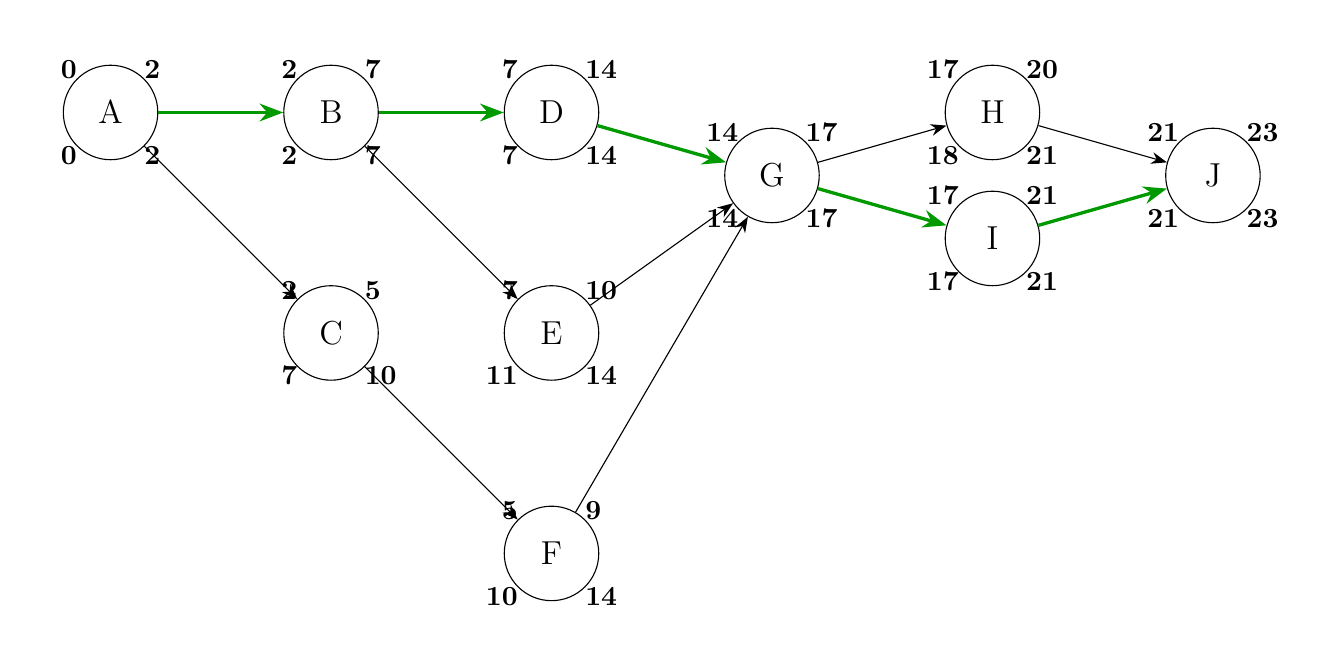
\begin{tikzpicture}[
    node distance=2.8cm,
    >=Stealth,
    activity/.style={
        circle,
        draw,
        minimum size=1.2cm,
        font=\large
    },
    crit/.style={very thick, -{Stealth[length=3mm]}, draw=green!60!black},
    normal/.style={-{Stealth[length=2mm]}},
    times/.style n args={4}{
        append after command={
           \pgfextra{
            \node[above left,  font=\bfseries, inner sep=12pt] at (\tikzlastnode) {#1};
            \node[above right, font=\bfseries, inner sep=12pt] at (\tikzlastnode) {#2};
            \node[below left,  font=\bfseries, inner sep=12pt] at (\tikzlastnode) {#3};
            \node[below right, font=\bfseries, inner sep=12pt] at (\tikzlastnode) {#4};
        }
        }
    },
    times/.default={0}{0}{0}{0}
]

% ROW 1

\node[activity, times={0}{2}{0}{2}] (A) {A};
\node[activity, times={2}{7}{2}{7}, right of=A] (B) {B};
\node[activity, times={2}{5}{7}{10}, below of=B] (C) {C};

% ROW 2
\node[activity, times={7}{14}{7}{14}, right of=B] (D) {D};
\node[activity, times={7}{10}{11}{14}, below of=D] (E) {E};
\node[activity, times={5}{9}{10}{14}, below of=E] (F) {F};

% ROW 3
\node[activity, times={14}{17}{14}{17}, right of=D, yshift=-0.8cm] (G) {G};

% ROW 4
\node[activity, times={17}{20}{18}{21}, right of=G, yshift=8mm] (H) {H};
\node[activity, times={17}{21}{17}{21}, right of=G, yshift=-8mm] (I) {I};

% ROW 5
\node[activity, times={21}{23}{21}{23}, right of=H, yshift=-8mm] (J) {J};

% --- ARROWS WITH DURATIONS ---
% From A
\draw[crit]   (A) --  (B);
\draw[normal] (A) --  (C);

% From B
\draw[crit]   (B) --  (D);
\draw[normal] (B) --  (E);

% From C
\draw[normal] (C) --  (F);

% From D
\draw[crit]   (D) --  (G);

% From E
\draw[normal] (E) --  (G);

% From F
\draw[normal] (F) -- (G);

% From G
\draw[normal] (G) -- (H);
\draw[crit]   (G) -- (I);

% From H
\draw[normal] (H) -- (J);

% From I
\draw[crit]   (I) -- (J);

\end{tikzpicture}
\caption{Activity on Node (AON) Diagram}
\end{figure}

\centering


\begin{description}
  \item[Forward Pass:] Definition of earliest start times based on earliest finish (EF) times.
  \begin{itemize}
      \item G: max( D\textsubscript{EF} = 14, E\textsubscript{EF} = 10, F\textsubscript{EF} = 9 ) = 14
      \item J: max( H\textsubscript{EF} = 20, I\textsubscript{EF} = 21 ) = 21
    \end{itemize}
    \item[Backward Pass:] Definition of latest finish times based on latest start (LS) times.
    \begin{itemize}
      \item G: min( H\textsubscript{LS} = 18, I\textsubscript{LS} = 17 ) = 17
      \item B: min( D\textsubscript{LS} = 7, E\textsubscript{LS} = 11 ) = 7
      \item A: min( B\textsubscript{LS} = 2, C\textsubscript{LS} = 7 ) = 2
    \end{itemize}
\end{description}


\paragraph{Critical Path:} A $\to$ B $\to$ D $\to$ G $\to$ I $\to$ J

\paragraph{Project duration:} 23 days

\end{landscape}







\newpage
\printbibliography
\nocite{*}

\end{document}
